%\documentclass{beamer}
\documentclass[xcolor=dvipsnames]{beamer}
\usepackage[latin1]{inputenc}
\usepackage{hyperref}
\usecolortheme[named=Violet]{structure}
\usetheme{Warsaw}
\usepackage{listings}
\usepackage{color}
\usepackage{framed}

\definecolor{dkgreen}{rgb}{0,0.6,0}
\definecolor{gray}{rgb}{0.5,0.5,0.5}
\definecolor{mauve}{rgb}{0.58,0,0.82}

% "define" julia
\lstdefinelanguage{julia}{morekeywords={function,if,else,while,for,:,end}, sensitive=true, morecomment=[l]{\#}, morecomment=[s]{/*}{*/}, morestring=[b]"}

% Default settings for code listings
\lstset{frame=tb,
   language=julia,
   aboveskip=3mm,
   belowskip=3mm,
   showstringspaces=false,
   columns=flexible,
   basicstyle={\small\ttfamily},
   numbers=none,
   frame=none,
   numberstyle=\tiny\color{gray},
   keywordstyle=\color{blue},
   commentstyle=\color{dkgreen},
   stringstyle=\color{mauve},
   breaklines=true,
   breakatwhitespace=true
   tabsize=3
}

\title[Scientific Computing]{Elements of Scientific Computing with Julia}
\begin{document}

\begin{frame}
\titlepage
\end{frame}

\AtBeginSubsection[]
{
  \begin{frame}<beamer>
    \frametitle{Today's Class}
    \tableofcontents[currentsection,currentsubsection]
  \end{frame}
}
\section{Recommender Systems}
\begin{frame}
{\bf Introduction}

{\it\huge I}n this lecture we are going to explore a further application of linear regression: Recommender Systems. \vfill
\pause

These are systems that allows businesses (or otherwise content providers) to more \emph{intelligently} provide their content based on their customers preferences.  \vfill

\pause 
For example: movie recommendations on Netflix or product recommendations on amazon.com.\\
\end{frame}

\begin{frame}
{\bf Main Types}
There are two main types of recommender systems:
\begin{enumerate}
\pause
\item \emph{Content based systems: }these are systems that base recommendations on the content of the media or information. For example, if you watch actions movies on Netflix and rate those positively, chances are that you will enjoy other action movies.
\pause
\item \emph{Collaborative filtering systems: }these are systems that base recommendations on similarities amongst users or customers. For example, if you bought a book on amazon that another user also bought along with other books, then maybe you would like those other books too.\\
\end{enumerate}
\end{frame}

\begin{frame}
Most recommender systems in use are based on these two main types or on some sort of hybrid of these types. \vfill\pause There are many techniques from scientific computing and machine learning that can be applied to implement these different types of recommender systems - such as \href{https://en.wikipedia.org/wiki/Singular_value_decomposition}{singular value decomposition} and \href{https://en.wikipedia.org/wiki/Cluster_analysis}{clustering analysis} (which are not covered in this course). \\
\end{frame}

\begin{frame}
Here, we will discuss simplified implementations of both content based and collaborative filtering systems that are basically applications of linear regression. \vfill\pause We will focus on algorithms that use gradient-based optimization (such as gradient descent or some more advanced optimization algorithm like \href{https://en.wikipedia.org/wiki/L-BFGS}{L-BFGS}) to find the least squares solution. \vfill\pause However, before we ``jump in'', let us take a detour through the topic of \emph{regularization}.\\
\end{frame}

\begin{frame}[fragile]
{\bf Regularization}
\emph{Regularization} refers to the technique of adding extra information to our linear (or logistic) regression in other to give preferential treatment to features that seem more relevantly correlated and penalize features whose correlation may not be that relevant to solving the regression.
\end{frame}

\begin{frame}
{\bf Regularized Cost Function and its Derivative}
\[
C(\theta) = \frac{1}{2m}\left[\sum_{i = 1}^m(h_{\theta}(x^{(i)}) - y^{(i)})^2 + \lambda\sum_{j=1}^n \theta_j^2\right]
\]
\pause
for $j=0$:
\[
\frac{\partial}{\partial \theta_0}C(\theta) = \frac{1}{m}\sum_{i=1}^m(h_{\theta}(x^{(i)})-y^{(i)})x^{(i)}_0
\]
\pause
for $j > 0$:
\[
\frac{\partial}{\partial \theta_j}C(\theta) = \frac{1}{m}\sum_{i=1}^m(h_{\theta}(x^{(i)})-y^{(i)})x^{(i)}_j + \frac{\lambda}{m}\theta_j
\]
\end{frame}

\begin{frame}
{\bf $\lambda$}
$\lambda$ is called the \emph{regularization parameter} - it is a parameter we should tweak in order to reward (or penalize) certain features. \vfill\pause Note that we do not regularize $\theta_0$ since it pertains to the ``ones'' feature and it is not affected by the weight of the features in consideration.
\end{frame}

\section{Content Based Systems}
\begin{frame}
{\bf Content Based Systems}

{\it\huge I}n content based systems, the \emph{features} which describe the content of something being recommended to users are known. \vfill\pause However, the user weights for these features are not known.\vfill\pause These features are information like amount of action or romance in a movie, or the different categories in which a particular product may fall. 
\end{frame}

\begin{frame}
{\bf Example}
For example, if you search for ``scientific computing'' on amazon.com, you will get a list of books that fall in that category. \vfill\pause
Clicking one of the results and scrolling down a bit, we find yet another example of content based recommendations:

\begin{center}
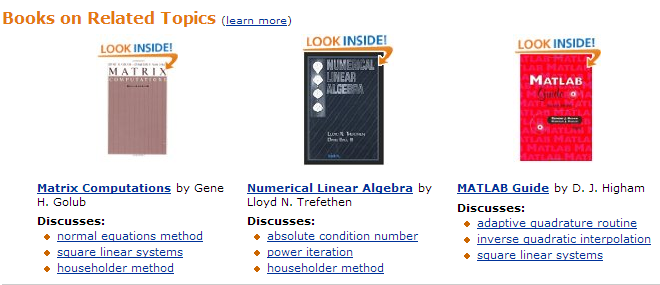
\includegraphics[scale=.5]{cb.png}
\end{center}
\end{frame}

\begin{frame}
{\bf A more simple example...}
In order to introduce the topic and formulate the problem, let us work on a simplified example:

\begin{center}
\begin{tabular}{| c | c | c | c | c |}
\hline
Book & Alice & Bob & Charlie & Dave \\
\hline
Advanced Math in Greek & 5 & 0 & 5 & 0\\
\hline
The Book of Proofs & ? & 2 & 5 & 0\\
\hline
Down-to-Earth Math & 0 & 5 & 1 & 4\\
\hline
Everyday Math & 0 & ? & ? & ? \\
\hline
Intermediate Crazy Math & 5 & 0 & ? & ?\\
\hline
\end{tabular}
\end{center}
\end{frame}

\begin{frame}
Say we have a matrix as above, where rows correspond to book tiles and columns correspond to readers (i.e. users of this system). \vfill\pause An entry $a_{i,j}$ in this matrix is a number ranging from 0 through 5, representing the rating user $j$ gave to book $i$. \vfill\pause If we do not have a rating from a particular user on a particular book, then the entry is represented by a ``?''. \\
\end{frame}

\begin{frame}
{\bf Definitions}
\begin{itemize}
\item $n_b$ is the number of books; \pause
\item $n_u$ is the number of users;\pause
\item $r(i,j) = 1$ if user $j$ has rated book $i$ (otherwise 0);\pause
\item $y^{(i,j)}$ is the rating by user $j$ of book $i$ if $r(i,j) = 1$;\pause
\item $\theta^{(j)}$ is the parameter vector for user $j$;\pause
\item $x^{(i)}$ is the feature vector for book $i$; and \pause
\item $(\theta^{(j)})^T(x^{(i)})$ is thus, the predicted rating for user $j$, for book $i$.\\
\end{itemize}
\end{frame}

\begin{frame}
{\bf Back to our Example}
Furthermore, in this case we know the feature vectors being considered: $x_1$ = amount of abstract mathematics and $x_2$ = amount of practical mathematics. \vfill\pause That is, someone read all of these books and ``graded'' them on these features, say on a scale from 0.0 to 1.0. \\
\end{frame}

\begin{frame}
{\bf Problem Formulation}
In order for us to learn $\theta^{(j)}$ (the parameter vector for user $j$ - or the weights user $j$ gives to the features considered) we must solve the following optimization problem:
\vfill\pause
\[
\boxed{\min_{\theta^{(j)}} \left(\frac{1}{2} \sum_{i:r(i,j)=1}((\theta^{(j)})^T(x^{(i)}) - y^{(i,j)})^2 + \frac{\lambda}{2}\sum_{k=1}^n(\theta^{(j)}_k)^2\right)}
\]\\
\end{frame}


\begin{frame}
{\bf Note ...}
The expression inside the parenthesis looks just like the regularized cost function we mentioned earlier, with the exception of the division by $m$. \vfill\pause Recall from our first discussion of linear regression that the $\frac{1}{m}$ constant multiplying our cost function was there for mathematical convenience and that it did not affect the minimum.\vfill\pause Here, the analogous constant factor would be $\frac{1}{m^{(j)}}$ where $m^{(j)}$ is the number of books rated by user $j$.\vfill\pause Since we will have to optimize for these $\theta^{(j)}$'s across all users $j$, then the constant factor $\frac{1}{m^{(j)}}$ is no longer convenient.\\
\end{frame}


\begin{frame}
{\bf Problem Formulation}
Thus to learn the parameters for all users $j$, that is $\theta^{(1)}, \theta^{(2)}, ..., \theta^{(n_u)}$, we need to solve:\vfill\pause

\begin{eqnarray*}
\min_{\theta^{(1)}, \theta^{(2)}, ..., \theta^{(n_u)}} \Bigg( \frac{1}{2} \sum_{j=1}^{n_u}\;\sum_{i:r(i,j)=1}((\theta^{(j)})^T(x^{(i)}) - y^{(i,j)})^2 \\ 
+ \frac{\lambda}{2}\sum_{j=1}^{n_u}\sum_{k=1}^n(\theta^{(j)}_k)^2 \Bigg)
\end{eqnarray*}

\end{frame}

\begin{frame}
{\bf Cost Function's Derivative}
If we are using a gradient based optimization algorithm to solve for the above problem, then we provide the derivative of the cost function:
\vfill\pause

For $k=0$ (since $j$ has a different meaning in our current formulation):
\[
\frac{\partial}{\partial \theta^{(j)}_0}C(\theta^{(j)}) = \sum_{i:r(i,j)=1}((\theta^{(j)})^T(x^{(i)}) - y^{(i,j)})x^{(i)}_0
\]
\vfill\pause

and for $k > 0$:
\[
\frac{\partial}{\partial \theta^{(j)}_k}C(\theta^{(j)}) = \sum_{i:r(i,j)=1}((\theta^{(j)})^T(x^{(i)}) - y^{(i,j)})x^{(i)}_k + \lambda\theta^{(j)}_k
\]
\end{frame}

\section{Collaborative Filtering Systems}
\begin{frame}
{\bf Collaborative Filtering Systems}

{\it\huge I}n collaborative filtering systems, the features which describe the content of something being recommended to users are not known. However, we do know the \emph{weights} users give to particular features. \vfill\pause For example, we know how Sally weighs her genre preferences when it comes to movies - we know that she really likes action movies, then ``contains action'' is a likely feature of the movies she watches.\\
\end{frame}

\begin{frame}
{\bf Example}

On the same amazon.com page I was before, we find an example of collaborative filtering:\vfill\pause

\begin{center}
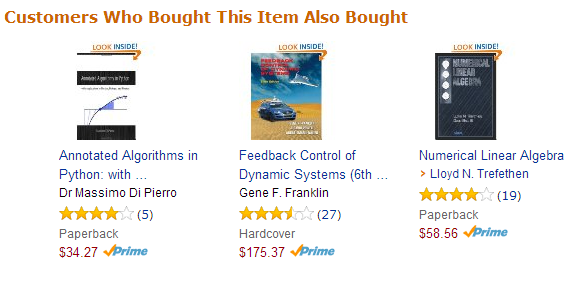
\includegraphics[scale=.5]{cf.png}
\end{center}
\end{frame}

\begin{frame}
{\bf A more simple example...}

Once again, let us work on a simplified example:

\begin{center}
\begin{tabular}{| c | c | c | c | c |}
\hline
Book & Alice & Bob & Charlie & Dave \\
\hline
Advanced Math in Greek & 5 & 0 & 5 & 0\\
\hline
The Book of Proofs & ? & 2 & 5 & 0\\
\hline
Down-to-Earth Math & 0 & 5 & 1 & 4\\
\hline
Everyday Math & 0 & ? & ? & ? \\
\hline
Intermediate Crazy Math & 5 & 0 & ? & ?\\
\hline
\end{tabular}
\end{center}
\end{frame}

\begin{frame}
This is the same matrix as before, however now we do not have any tags on these books, i.e. there is no ``grade'' for the amount of abstract mathematics versus practical mathematics. \vfill\pause However, we do have the following weight vectors for each user, say:
\vfill\pause
$\theta^{(1)} = \begin{bmatrix}
0\\ 5\\ 0
\end{bmatrix}, \; \theta^{(2)} = \begin{bmatrix}
0\\ 1\\ 5
\end{bmatrix}, \; \theta^{(3)} = \begin{bmatrix}
0\\ 5\\ 0
\end{bmatrix}, \; \theta^{(4)} = \begin{bmatrix}
0\\ 0\\ 5
\end{bmatrix}$\\
\end{frame}

\begin{frame}
{\bf Problem Formulation}
The definitions for the notation we will use here are the same as before. \vfill\pause So given vectors $\theta^{(j)}$'s for all $n_u$ users, we wish to learn the vector $x^{(i)}$ (the feature vector for book $i$). \vfill\pause Thus, we must solve the following optimization problem:
\vfill\pause
\[
\boxed{\min_{x^{(i)}} \left(\frac{1}{2} \sum_{j:r(i,j)=1}((\theta^{(j)})^T(x^{(i)}) - y^{(i,j)})^2 + \frac{\lambda}{2}\sum_{k=1}^n(x^{(i)}_k)^2\right)}
\]\\
\end{frame}

\begin{frame}
{\bf Problem Formulation}
In order to learn the features for all books $i$, that is $x^{(1)}, x^{(2)}, ..., x^{(n_b)}$, we need to solve:
\vfill\pause
\begin{eqnarray*}
\min_{x^{(1)}, x^{(2)}, ..., x^{(n_b)}} \Bigg(\frac{1}{2} \sum_{i=1}^{n_b}\;\sum_{j:r(i,j)=1}((\theta^{(j)})^T(x^{(i)}) - y^{(i,j)})^2 \\ + \frac{\lambda}{2}\sum_{i=1}^{n_b}\sum_{k=1}^n(x^{(i)}_k)^2\Bigg)
\end{eqnarray*}
\end{frame}

\begin{frame}
{\bf Cost Function's Derivative}
If we are using a gradient based optimization algorithm to solve for the above problem, then the derivative of the cost function here should be with respect to $x^{(i)}$, \vfill\pause however it should not look too different from before and working the differentiation is left to you as an exercise.\\
\end{frame}

\begin{frame}
{\bf Going back and forth...}
So once we solve the above problem and get a good approximation of $x^{(1)}, x^{(2)}, ..., x^{(n_b)}$, there is no reason why we can't use this new information to estimate $\theta^{(1)}, \theta^{(2)}, ..., \theta^{(n_u)}$ \vfill\pause - as we might not have all of them, or there may be new users over time. \vfill\pause But there may also be new books over time, and we can go back and forth in this manner estimating features and parameters. \\
\end{frame}

\begin{frame}
{\bf Look carefully...}
If you study the two minimization problems below, you will see that it is possible to combine them into one: \vfill\pause

In order to learn the features for all books $i$ we need to solve:
\[
\min_{x^{(1)}, x^{(2)}, ..., x^{(n_b)}} \left(\frac{1}{2} \sum_{i=1}^{n_b}\;\sum_{j:r(i,j)=1}((\theta^{(j)})^T(x^{(i)}) - y^{(i,j)})^2 + \frac{\lambda}{2}\sum_{i=1}^{n_b}\sum_{k=1}^n(x^{(i)}_k)^2\right)\]

\vfill\pause
And in order to learn the parameters for all users $j$ we need to solve:
\[
\min_{\theta^{(1)}, \theta^{(2)}, ..., \theta^{(n_u)}} \left(\frac{1}{2} \sum_{j=1}^{n_u}\;\sum_{i:r(i,j)=1}((\theta^{(j)})^T(x^{(i)}) - y^{(i,j)})^2 + \frac{\lambda}{2}\sum_{j=1}^{n_u}\sum_{k=1}^n(\theta^{(j)}_k)^2\right)\]
\end{frame}

\begin{frame}
{\bf Combining the Problems}
... combined, becomes:
\begin{eqnarray*}
\min_{x^{(1)}, x^{(2)}, ..., x^{(n_b)}, \theta^{(1)}, \theta^{(2)}, ..., \theta^{(n_u)}} \Bigg(\frac{1}{2} \sum_{(i,j):r(i,j)=1}((\theta^{(j)})^T(x^{(i)}) - y^{(i,j)})^2 \\ + \frac{\lambda}{2}\sum_{i=1}^{n_b}\sum_{k=1}^n(x^{(i)}_k)^2 + \frac{\lambda}{2}\sum_{j=1}^{n_u}\sum_{k=1}^n(\theta^{(j)}_k)^2\Bigg)
\end{eqnarray*}
\end{frame}

\begin{frame}
{\bf Collaborative Filtering Algorithm}
\begin{enumerate}
\item Initialize $x^{(1)}, x^{(2)}, ..., x^{(n_b)}, \theta^{(1)}, \theta^{(2)}, ..., \theta^{(n_u)}$ to small random numbers.\vfill\pause
\item Minimize the cost function 
\[C(x^{(1)}, x^{(2)}, ..., x^{(n_b)}, \theta^{(1)}, \theta^{(2)}, ..., \theta^{(n_u)})\]
using gradient descent or another optimization algorithm.\vfill\pause
\item For a user $j$ with parameters $\theta^{(j)}$ and for a book $i$ with features $x^{(i)}$, predict a rating of $(\theta^{(j)})^T(x^{(i)})$.
\end{enumerate} 
\vfill\pause
The algorithm just described here is also known as \emph{low-rank matrix factorization}.
\end{frame}

\begin{frame}
{\bf Top 10}
We can use the results to find the top ten similar books to some book $i$ as follows: \vfill\pause find the ten books $l$ with the smallest distance from book $i$, that is $||x^{(i)} - x^{(l)}||$.
\end{frame}

\end{document}